\newcommand{\fourier}[1]{\ensuremath{\mathcal{F}\left\{#1\right\}}}
\newcommand{\ifourier}[1]{\ensuremath{\mathcal{F}^{-1}\left\{#1\right\}}}
\newcommand{\intwhole}{\ensuremath{\int_{-\infty}^{+\infty}}}
\newcommand{\sumwhole}[1]{\ensuremath{\sum_{#1=-\infty}^{+\infty}}}
\chapter{Campionamento e Ricostruzione con Quasirandom Number Generation}\label{chapter5}
La funzione immagine definita sull'Image plane \`e una funzione continua, ma l'output del sistema di rendering \`e una griglia 2D di punti colorati. 
Scegliere accuratamente la strategia di 
campionamento dal film plane \`e fondamentale per migliorare la qualit\`a del risultato finale.\par
Al fine di poter formalizzare il processo di scelta di campioni dal film plane\footnote{Sinonimo di Image plane, nomenclatura introdotta da 
\cite{pharr}} e valutazione della funzione continua dai campioni (Ricostruzione),
si richiamano di seguito due distinte teorie: 
\begin{altDescription}{Sampling}
	\item[Analisi di Fourier del Segnale] Possiamo analizzare in frequenza la varianza di una strategia di campionamento. In particolare, 
		analizzandone il suo spettro di potenza, \`e possibile analizzare quali frequenze contribuiscono maggiormente alla varianza stessa. Affinch\`e 
		l'immagine finale risulti di qualit\`a, \`e desiderabile per una strategia di campionamento presentare varianza quasi nulla o nulla per le 
		basse frequenze.\\ Un esempio di tale analisi \`e mostrato in Figura \ref{chapter5:sampling:owen}
	\item[Quasirandom Number Generation] Al fine di migliorare la copertura dello spazio campionario dei campioni generati, ci si pu\`o affidare 
		a sequenze deterministiche minimizzanti una metrica chiamata \textit{Discrepancy}, definita nelle sezioni successive
\end{altDescription}
Si precisa infine che la parola "pixel" \`e usata in due contesti differenti
\begin{itemize}[topsep=0pt,noitemsep]
	\item[] Un \textit{Display Pixel} \`e un elemento fisico di un display che emette luce di un determinato colore
	\item[] Un \textit{Image Pixel} \`e un \textit{campione puntiforme privo di area} della funzione immagine filtrata $r_f(x,y)$, i quali 
		definiscono il valore del display pixel integrando una cella definita da quest'ultimo
\end{itemize}
\section{Campionamento}
\subsection{Richiami Fourier Analysis}
L'analisi di Fourier \`e usata per valutare la qualit\`a del segnale ricostruito rispetto all'uriginale. La \textit{Trasformazione di Fourier} 
consiste nella scomposizione di una funzione continua in un integrale di sinusoidi pesate, le cui ampiezze e fasi costituiscono una funzione complessa 
a valori reali (frequenza), la trasformata secondo Fourier. Possiamo trasformare tale trasformata dal dominio delle frequenze al dominio di partenza 
applicando la \textit{Trasformazione inversa di Fourier}. Tale coppia di trasformazioni \`e definita come 
\begin{align}
	F(\nu)&=\fourier{f(x)}=\int_{-\infty}^{+\infty}f(x)e^{-\iota 2\pi \nu x}\mathrm{d}x \\
	f(x)&=\ifourier{F(\nu)}=\int_{-\infty}^{+\infty}F(\nu)e^{\iota 2\pi \nu x}\mathrm{d}\nu
\end{align}
Le quali possono essere estese a domini multidimensionali applicando la trasformazione a ciascuna coordinata singolarmente
\begin{align}
	F(\nu_1,\ldots,\nu_d)&=\fourier{f(x_1,\ldots,x_d)}\nonumber\\ 
		&=\int_{-\infty}^{+\infty}\cdots\left(
		\int_{-\infty}^{+\infty}f(x_1,\ldots,x_d)e^{-\iota 2\pi \nu_1 x_d}\mathrm{d}x_1\right)\ldots e^{-\iota 2\pi \nu_d x_d}\mathrm{d}x_d \\
	f(x_1,\ldots,x_d)&=\ifourier{F(\nu_1,\ldots,\nu_d)} \nonumber\\
		&=\int_{-\infty}^{+\infty}\cdots\left(\int_{-\infty}^{+\infty}
		F(\nu_1,\ldots,\nu_d)e^{\iota 2\pi \nu_1 x_1}\mathrm{d}\nu_1\right)\ldots e^{\iota 2\pi \nu_dx_d}\mathrm{d}\nu_d
\end{align}
Le seguenti generalizzazioni dunque valgono anche per segnali multidimensionali.
La formalizzazione del processo di campionamento (ideale) con periodo $T$ \`e data dalla moltiplicazione di una funzione continua per un 
treno di impulsi $\sha_T(x)=T\sum_{i=-\infty}^{\infty}\delta(x-iT)$,
\begin{equation}
	f(x)\sha_T(x)=Tf(x)\sum_{i=-\infty}^{\infty}\delta(x-iT)=\sum_{i=-\infty}^{\infty}f[i]\delta(x-iT)
\end{equation}
dove $f[i]=Tf(iT)$ segnale tempo discreto campionato con periodo $T$\par
Tale espressione nel dominio della frequenza consiste in una somma di repliche del segnale originale
\begin{align}
	\fourier{f(x)\sha_T(x)}&=F(\nu)*T\sha_{1/T}(\nu) \nonumber\\
		&=\intwhole F(u)T\sha_{1/T}(\nu-u)\mathrm{d}u \nonumber\\
		&=\intwhole F(u)\sumwhole{k}\delta\left(\nu-u+\frac{k}{T}\right)\mathrm{d}u \nonumber\\
		&=\sumwhole{k}\intwhole F(u)\delta\left(\nu-u+\frac{k}{T}\right)\mathrm{d}u \nonumber\\
		&=\sumwhole{k}F\left(\nu-u+\frac{k}{T}\right)
\end{align}
Da cui si enuncia il fondamentale \textit{Teorema di Shannon} del campionamento \cite{pegoraro}
\begin{theoremS}
	Sia $F(\nu)$ segnale a banda limitata, \mbox{$\exists \nu_b\in\mathbb{R}^+\backepsilon^\prime\;F(\nu)=0\;\forall |\nu|>\nu_b$}, il 
	\textit{Teorema del campionamento di Nyquist-Shannon} afferma che tale segnale \`e perfettamente costruibile dai suoi samples, quando \`e 
	soddisfatto il \textit{Nyquist Criterion} $\tfrac{\nu_s}{\nu_b}>2$, cio\`e se la frequenza di campionamento $\nu_s$ \`e pi\`u grande del 
	\textit{Nyquist Rate} $2\nu_b$, o equivalentemente quando la frequenza limite di banda $\nu_b$ \`e inferiore della \textit{Nyquist Frequency} 
	$\tfrac{\nu_s}{2}$
\end{theoremS}
La distanza tra bande successive \`e incrementata aumentando la frequenza di campionamento $\nu_s$, processo detto \textit{oversampling} di un fattore 
$N>1$ se $\tfrac{\nu_s}{\nu_b}>2N$, il che permette ai filtri (dopo) di avere una banda di transizione pi\`u variabile. Al contrario, 
\textit{undersampling} consiste nel campionare con frequenza $\nu_s$ tale che $N\leq0$, il che significa che il teorema del campionamento non \`e 
soddisfatto, generando la sovrapposizione delle repliche scalate degli spettri del segnale originale in frequenza, non permettendo la ricostruzione 
(dopo), il che provoca il fenomeno noto come \textit{Aliasing}, il che si pu\`o manifestare in immagini statiche come \textit{pattern di Moir\'{e}}
ed in animazioni come \textit{wagon-wheel effect}. Con pi\`u precisione, ci si riferisce con \textit{Pre-Aliasing} agli artefatti di aliasing 
introdotti dal campionamento e con \textit{Post-Aliasing} agli artefatti di aliasing introdotti dalla ricostruzione. Non sempre si pu\`o aumentare 
la frequenza di campionamento per migliorare la qualit\`a dell'immagine, in quanto si rischia di incorrere in costi elevati di computazione.\par
Si noti che segnali reali mai sono banda limitata, per la presenza di discontinuit\`a.\par
Data una sequenza di campioni, campionata con frequenza di campionamento $\nu_s=T^{-1}$, che soddisfa il teorema di Shannon $f[i]$, essa pu\`o 
essere utilizzata per ricostruire la funzione originare con l'\textit{interpolazione ideale di Shannon-Whittaker}
\begin{equation}
	f(x)=\sumwhole{j}\operatorname{sinc}(x-kT)f[k]
\end{equation}
Il che \`e equivalente ad applicare un filtro passa basso di estensione pari alla banda limite del segnale $\nu_b$. Tale funzione non \`e utilizzata 
nella pratica per lo svantaggio di dover valutare tutti i campioni per la ricostruzione in ogni singolo punto della funzione. Preferiamo metodi che 
permettono di ricostruire la funzione originale valutandola in un intorno del punto di valutazione, ed \`e per questo che applichiamo un filtro di 
ricostruzione.\par
Ricordiamo la definizione di \textit{Power Spectral Density}, per un segnale con energia 
\begin{align}
	S_f(\nu)&=\lim_{T\to\infty}\frac{1}{T}|\fourier{f_T(x)}|^2\\
	f_T(x)&=\left\{\begin{aligned}
		&f(x)\;&\mathrm{se}\;x\in[-T,T]\nonumber\\
		&0&\mathrm{altrimenti}\nonumber
	\end{aligned}\right.\nonumber
\end{align}
Tipicamente, per segnali che sono campionati e processati nel dominio tempo-discreto, utilizziamo una seconda definizione, che pu\`o essere ottenuta 
da questa campionando il segnale e prendendo il limite $T_s\to0$
\begin{equation}
	S_f(\nu)=F(\nu)\xoverline{F(\nu)}
\end{equation}
Tale concetto \`e utile per analizzare statisticamente un Sampling pattern. Talvolta un PSD per un sampling pattern pu\`o essere derivata 
analiticamente, come per il campionamento uniforme \cite{pharr}, altre va calcolato numericamente, come per sampling stocastico.\par
In generale, L'\textit{aliasing \`e ridotto se la PSD di una strategia di campionamento \`e minima alle basse frequenze}
\subsection{Quasirandom Number Generation}\label{chapter5:sampling:QuasiMonteCarlo}
Un altro concetto al di fuori della Fourier Analysis per valutare la qualit\`a di samples \`e il concetto di \textit{Discrepancy}. La generazione di 
sequenze di numeri a bassa discrepanza ha lo scopo di costruire delle formule matematiche (deterministiche) per campionare punti all'apparenza 
casuali con migliore uniformit\`a e copertura del dominio che si ottiene con un campionatore uniforme. La Discrepanza infatti \`e una metrica che 
misura quanto uniformemente una data successione copre un dato spazio campionario.\par
(\cite{pharr}) L'idea \`e quella di suddividere\footnotemark{} un dominio d-dimensionale $[0,1)^d$ in tante regioni, contare il numero di punti in 
ciascuna regione, e comparare tale numero $\norm{\{x_i\in b\}}$ alla frazione di volume della regione $V(b)$. La frazione di punti rispetto al numero 
di campioni totali di una data regione dovrebbe essere proporzionale alla percentuale di volume totale della regione.\par
\footnotetext{Per suddivisione non si intende una partizione del volume totale, ma sottoinsiemi arbitrari di esso la cui unione \`e il volume totale}
Scegliamo come suddivisione di $[0,1)^d$ una famiglia di parallelepipedi con un vertice sull'origine
\begin{equation}
	B=\{[0,v_1]\times [0,v_2]\times\cdots\times [0,v_d]\}
\end{equation}
Da cui, dati $n$ samples $P=\{x_1,\ldots,x_n\}$, la \textit{discrepancy} di $P$ rispetto a $B$ \`e definita come
\begin{equation}
	D_n(B,P)=\stackrel[{b\in B}]{}{\operatorname{sup}}\left\vert\frac{\norm{\{x_i\in b\}}}{n}-V(b)\right\vert
\end{equation}
In particolare, quando la famiglia di volumi scelta per calcolare la \textit{discrepancy} \`e l'insieme di parallelepipedi con centro l'origine, 
il valore che \`e calcolato \`e anche chiamato \textit{Star Discrepancy}.\par
Tale valore pu\`o essere calcolato in modo analitico per alcuni particolari insiemi di punti. Consideriamo infatti $n$ punti equispaziati, 
$x_i=\frac{i}{n}$. Scegliendo come famiglia di volumi 
\begin{equation*}
	B_u=\left\{\left[0,\frac{1}{n}\right),\left[0,\frac{2}{n}\right),\ldots,\left[0,1\right)\right\}
\end{equation*}
Si ottiene star discrepancy
\begin{equation}
	D_n^*(\{x_i\}_{i=1}^n,B_u)=\frac{1}{n}
\end{equation}
Una sequenza di punti d-dimensionale \`e a bassa discrepanza se la sua \textit{star discrepancy} \`e dell'ordine 
\mbox{$\mathcal{O}\left(\frac{(\log n)^d}{n}\right)$}
\subsection{Halton Sampler}
Tra i vari campionatori esistenti (\cite{pharr}, \cite{pegoraro}, \cite{akenine-moller}), analizziamo con i due framework brevemente spiegati in 
precedenza, il campionatore basato sulla quasirandom \textit{Sequenza di Halton}. Tale sequenza \`e costruita utilizzando 
l'\textit{Inverso Radicale}:\\
Un numero positivo \`e esprimibile in base $b$ come somma di cifre 
\begin{equation}
	a=\sum_{i=1}^{m}d_i(a)b^{i-1},\;d_i(a)\in[0,1)
\end{equation}
La Funzione Inverso Radicale $\Phi_b$ in base $b$ converte un intero nonnegativo in una frazione $\in[0,1)$ riflettendo le cifre del numero di 
partenza rispetto al punto
\begin{equation}
	\Phi_b(a)=0.d_1(a)d_2(a)\ldots d_m(a)=\sum_{i=1}^md_i(a)b^{-i}
\end{equation}
Un campionatore d-dimensionale pu\`o essere costruito scegliendo per ogni dimensione una funzione inverso radicale con base pari ad un numero primo. 
La generazione di $n$ campioni consiste nel valutare tali funzioni per $0,1,\ldots,n-1$
\begin{equation}
	x_a=(\Phi_2(a),\Phi_(3),\ldots,\Phi_{p_d}(a))
\end{equation}
La star discrepancy della sequenza ottenuta \`e pari a \mbox{$D_n^*(x_a,B_u)=\mathcal{O}\left(\frac{(\log n)^d}{n}\right)$}, cio\`e il valore ottimale.
Si noti che l'implementazione del calcolo di tali radicali \`e mantenuto con aritmetica intera per evitare di accumulare errore di round-off.\par
Uno svantaggio di tale sequenza (\cite{pharr}) \`e che \`e deterministica, dunque non ne possiamo valutare la varianza di un integrale stimato con 
essa. Inoltre, man mano che la base cresce, la sequenza diventa sempre pi\`u regolare, rendendo basi alte inutilizzabili. Per risolvere tali problemi
si pu\`o attuare una permutazione casuale, diversa per ogni cifra, affinch\`e tali permutazioni generino una sequenza che approcci una distribuzione 
uniforme. Tale processamento dei punti della sequenza di Halton \`e chiamata \textit{Scrambling}.\par
In particolare, una strategia di Scrambling efficace per la sequenza di Halton \`e l'\textit{Owen Scrambling} \cite{pharr}, per il quale si pu\`o
dimostrare diminuire l'andamento asintotico dell'errore di integrazione a
\begin{equation}
	\mathcal{O}\left(n^{-\frac{3}{2}}(\log n)^{\frac{d-1}{2}}\right)
\end{equation}
\begin{figure}[tb]
	\centering
	\begin{subfigure}[t]{0.4\linewidth}
		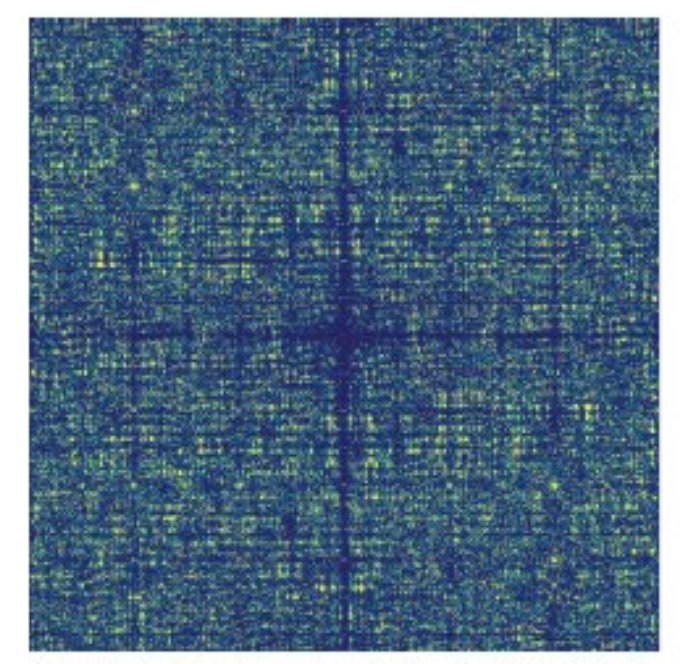
\includegraphics[width=\linewidth]{../assets/chapter5_sampling_haltonPSD.png}
		\caption{Senza Owen Scrambling. Prestazioni migliori rispetto al campionamento uniforme, in quanto presenta contributi minimi alle basse 
			frequenze, ma contiene eccessiva variazione nelle alte frequenze}
		\label{chapter5:sampling:owen:no}
	\end{subfigure}
	\begin{subfigure}[t]{0.5\linewidth}
		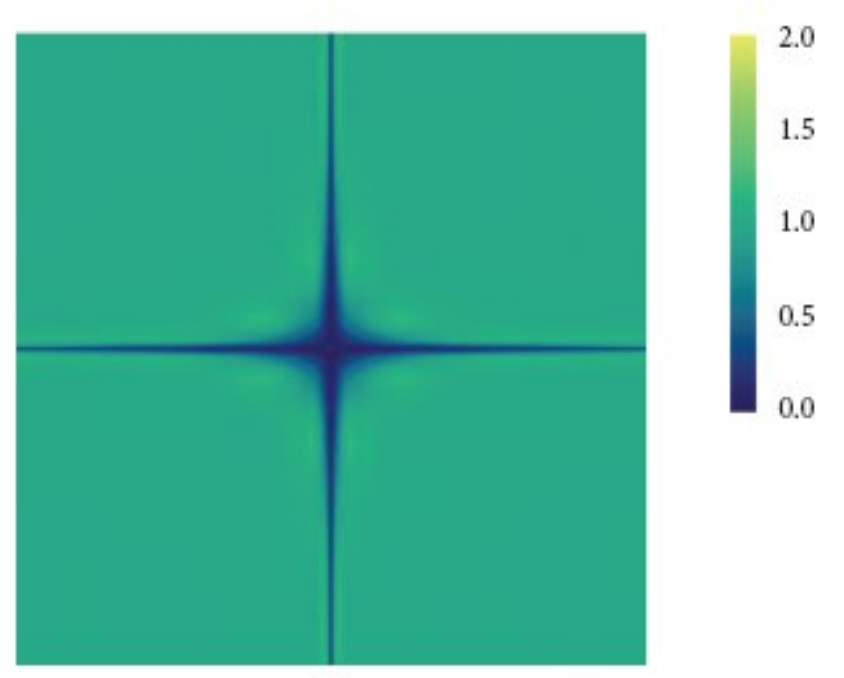
\includegraphics[width=\linewidth]{../assets/chapter5_sampling_owenPSD.png}
		\caption{Con Owen Scrambling. PSD quasi unitaria nella maggior parte del dominio alle alte frequenze.}
		\label{chapter5:sampling:owen:yes}
	\end{subfigure}
	\caption{Illustrazione delle Power Spectral Densities del campionatore basato sulla sequenza di Halton con basi 2 e 3, con e senza Owen Scrambling.
		Immagini da \cite{pharr}}
	\label{chapter5:sampling:owen}
\end{figure}
Il che \`e superiore all'$\mathcal{O}(n^{-1/2})$ per Monte Carlo con punti campionati uniformemente.\par
Lo Scrambling per l'n $i$-esima coordinata del $k$-esimo punto della sequenza $x_k^{(i)}=0.d_1d_2\ldots d_m$ \`e mostrato in 
\ref{appendixD:owenScrambling} con codice C\texttt{++} ripreso da \cite{pharr} e commentato.
\begin{figure}[b]
	\centering
	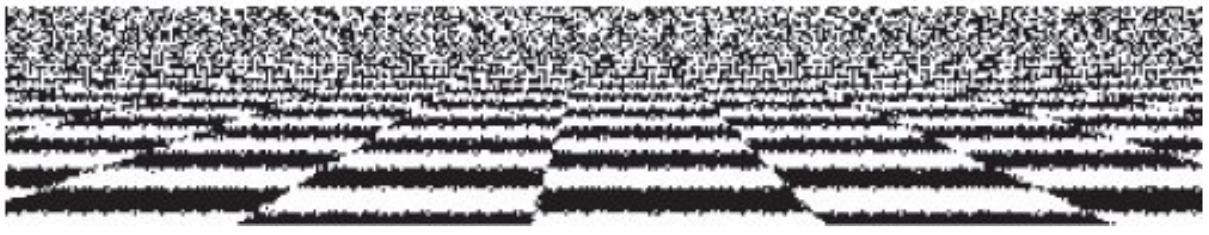
\includegraphics[width=\linewidth]{../assets/chapter5_sampling_result.png}
	\caption{Risultato dell'applicazione del campionamento con Scrambled Halton Sequence. Immagine da \cite{pharr}}
	\label{chapter5:sampling:result}
\end{figure}
\section{Ricostruzione}
Un segnale continuo pu\`o essere ricostruito dai suoi campioni (perfettamente o meno) con una moltiplicazione nel dominio della frequenza con la 
funzione di trasferimento di un \textit{filtro di ricostruzione} $F_r$, o equivalemntemente con la convoluzione del segnale a dominio discreto 
rappresentato dai campioni con la risposta all'impulso del filtro, $f_r$. Ricordiamo che le immagini che andiamo a campionare non sono a banda
limitata, in quanto presentano discontinuit\`a. L'obiettivo \`e dunque trovare una strategia che permetta di minimizzare l'errore tra la funzione 
ricostruita e la funzione originale.\par
Il filtro ideale risulta non essere una scelta appropriata (\cite{pharr}), in qunato esso \`e affetto dal problema del \textit{ringing} per funzioni
oltre la \textit{nyquist frequency}, ci\`o vuol dire che i bordi degli gli oggetti risultano replicati nei pixel vicini (pi\`u formalmente noto come 
Fenomeno di Gibbs). Inoltre, $\operatorname{sinc}$ ha estensione infinita, in quanto non va a zero per un valore finito della distanza.\par
Si noti che i filtri di seguito descritti saranno 1D, ma da essi possiamo costruire un filtro d-dimensionale in due modi:\\
Costruendo un \textit{filtro separabile} (si veda \ref{chapter5:reconstruction:boxFilter})
\begin{equation}
	f(x,y)=f(x)f(y)
\end{equation}
Il cui campionamento pu\`o essere compiuto integrando in ogni quadrante, supponendo $f$ simmetrica
\begin{equation}
	4\int_0^{y_s}\int_0^{x_s}f(x,y)\mathrm{d}x\mathrm{d}y = \left(2\int_0^{x_s}f(x)\mathrm{d}x\right)\left(2\int_0^{y_s}f(y)\mathrm{d}y\right)
\end{equation}
da cui basta applicare Inverse Transform Sampling alla CDF definita da ciascuno degli integrali monodimensionali. Inoltre, per scalare tale 
filtro per $t=Tx$, basta sostituire
\begin{equation}
	2\int_0^{t_s}\frac{1}{|T|}f\left(\frac{t}{T}\right)\mathrm{d}t=2\int_0^{\frac{t_s}{T}}f(t)\mathrm{d}t
\end{equation}
La seconda scelta per costruire un filtro bidimensionale da uno monodimensionale \`e un \textit{filtro radiale}
\begin{align}
	f(x,y)&=\frac{f(\rho)}{2\pi c},\\
	\rho &= \sqrt{x^2+y^2}\nonumber\\
	c &= \int_0^{\infty}\rho f(\rho)\mathrm{d}\rho\nonumber
\end{align}
Per il quale, seguendo ragionamento analogo al precedente \cite{pegoraro}, possiamo applicare inverse transform sampling
\begin{equation}
	\int_0^{\rho_s}\frac{1}{T|T|}\frac{1}{c}f\left(\frac{\rho}{T}\right)\rho\mathrm{d}\rho=\int_0^{\frac{\rho_s}{T}}\frac{1}{c}f(\rho)\rho\mathrm{d}\rho
\end{equation}
\subsection{Box Filter}\label{chapter5:reconstruction:boxFilter}
Uno dei filtri pi\`u comunemente usati \`e il box filter, il quale rappresenta effettivamente il risultato "standard", utilizzato ad esempio per 
comparare campionatori. Essendo il pi\`u semplice dei filtri, il quale ricostruisce una funzione piecewise constant, introduce post aliasing, anche 
se il campionamento \`e effettuato con un elevata sampling frequency.
\begin{align}
	f(x)=\sqcap(x)=\left\{\begin{aligned}
		&1 &\mathrm{se}\;|x|<\tfrac{1}{2}\\
		&\tfrac{1}{2}\;&\mathrm{se}\;|x|=\tfrac{1}{2}\\
		&0 &\mathrm{se}\;|x|>\tfrac{1}{2}
	\end{aligned}\right.
\end{align}
Il quale ha funzione di trasferimento
\begin{equation}
	F(\nu)=\operatorname{sinc}(\pi\nu)
\end{equation}
Utilizzandolo in due dimensioni come un filtro separabile esso ha espressione \mbox{$f(x,y)=\sqcap(x)\sqcap(y)$} con 
integrale pari a $4x_by_b$, dove $x_b$ e $y_b$ semiestensioni del filtro, e funzione di trasferimento
\mbox{$F(\nu_x)*F(\nu_y)$}\par
Nel caso in cui si utilizzi il box filter come filtro radiale, 
\begin{equation}
	f(x,y)=f\left(\tfrac{r}{c}\right)
\end{equation}
\begin{figure}[tb]
	\centering 
	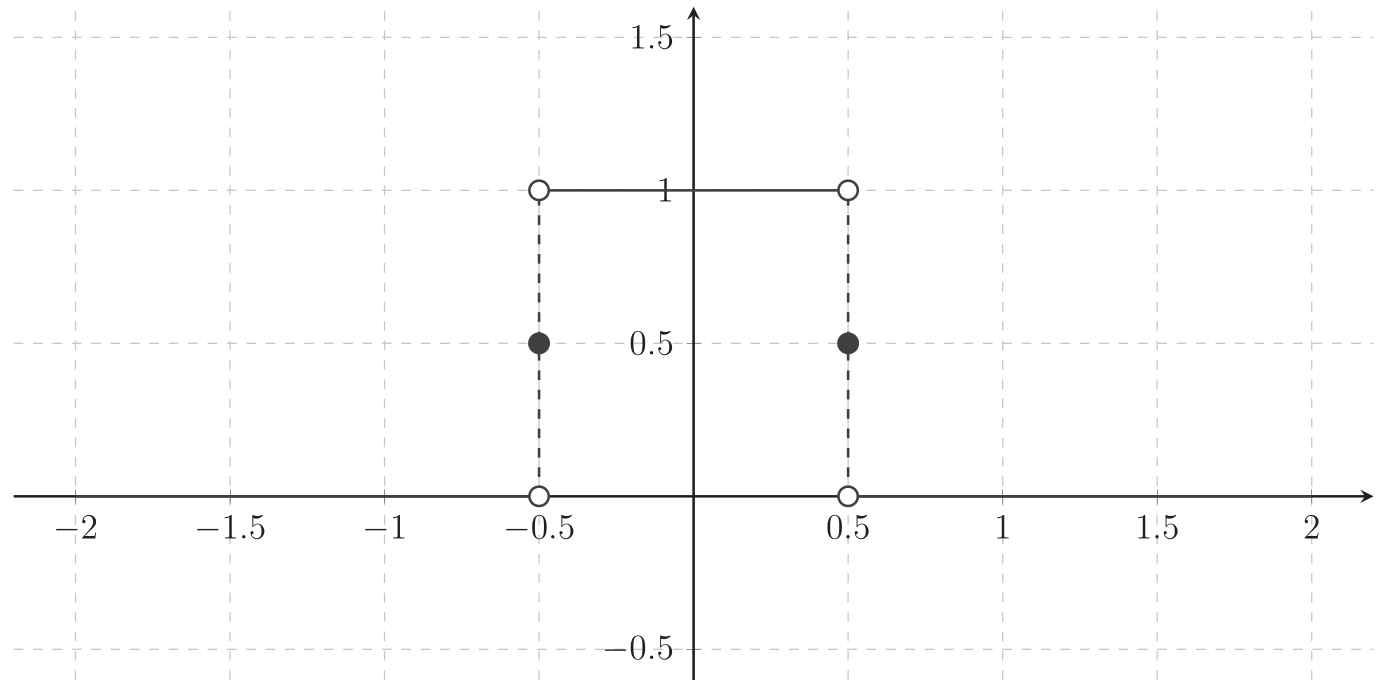
\includegraphics[width=0.8\linewidth]{../assets/chapter5_reconstruction_box.png}
	\caption{Illustrazione della risposta all'impulso del box filter. Immagine da \cite{pegoraro}}
	\label{chapter5:reconstruction:boxFilter}
\end{figure}
dove $c$ semiestensione del filtro. Esso ha funzione di trasferimento
{
	\newcommand{\eq}{\stackrel{\small{\theta=\varphi-\phi}}{=}}
	\newcommand{\eqa}{\mathmakebox[\widthof{x=x-x}]{=}}
\begin{align}
	F(\nu_x,\nu_y)&\eqa\intwhole\intwhole f(x,y)e^{-\iota 2\pi(\nu_xx + \nu_yy)}\mathrm{d}x\mathrm{d}y \nonumber\\
	&\eqa\int_0^{2\pi}\int_0^{\infty}f\left(\tfrac{r}{c}\right)e^{-\iota 2\pi r \rho\cos(\varphi-\phi)}r\mathrm{d}r\mathrm{d}\varphi\nonumber\\
	&\eq\int_0^{\infty}f\left(\tfrac{r}{c}\right)\int_{-\phi}^{2\pi-\phi}e^{-\iota 2\pi r\rho\cos\theta}\mathrm{d}\theta r\mathrm{d}r\nonumber\\
	&\eqa2\pi\int_0^{\infty}f\left(\tfrac{r}{c}\right)J_0(2\pi r\rho)r\mathrm{d}r\nonumber \\
	&\eqa 2\pi\int_0^{\tfrac{c}{2}}J_0(2\pi r\rho)r\mathrm{d}r\stackrel{\uptau=2\pi r\rho}{=}\frac{1}{2\pi\rho^2}\int_0^{c\pi\rho}
		J_0(\uptau)\uptau\mathrm{d}\uptau\nonumber\\
	&\eqa\frac{c}{2\rho}J_1(c\pi\rho)
\end{align}
}
Per campionare il filtro separabile (vedi Equazione \ref{chapter2:camera:weightEstimatorOne}), la CDF della box function \`e pari a 
\begin{equation}
	2\int_0^{x_s}\sqcap(x)\mathrm{d}x=2\int_0^{x_s}=2x_s
\end{equation}
Dunque possiamo applicare Inverse transform sampling, dato un $\xi\sim\mathcal{U}(0,1)$, 
\begin{equation}
	\xi=2x_s\longrightarrow x_s=\frac{x_s}{2}
\end{equation}
Seguito da una scala per il dominio di interesse. Nel filtro radiale, la CDF
\begin{equation}
	8\int_0^{\rho_s}\sqcap(\rho)\rho\mathrm{d}\rho=8\int_0^{\rho_s}\rho\mathrm{d}\rho=4\rho_s^2
\end{equation}
Da cui si pu\`o applicare Inverse Transform Sampling
\begin{equation}
	\xi=4\rho_s^2\longrightarrow\rho_s=\frac{\sqrt{\xi}}{2}
\end{equation}
\begin{figure}[tb]
	\centering
	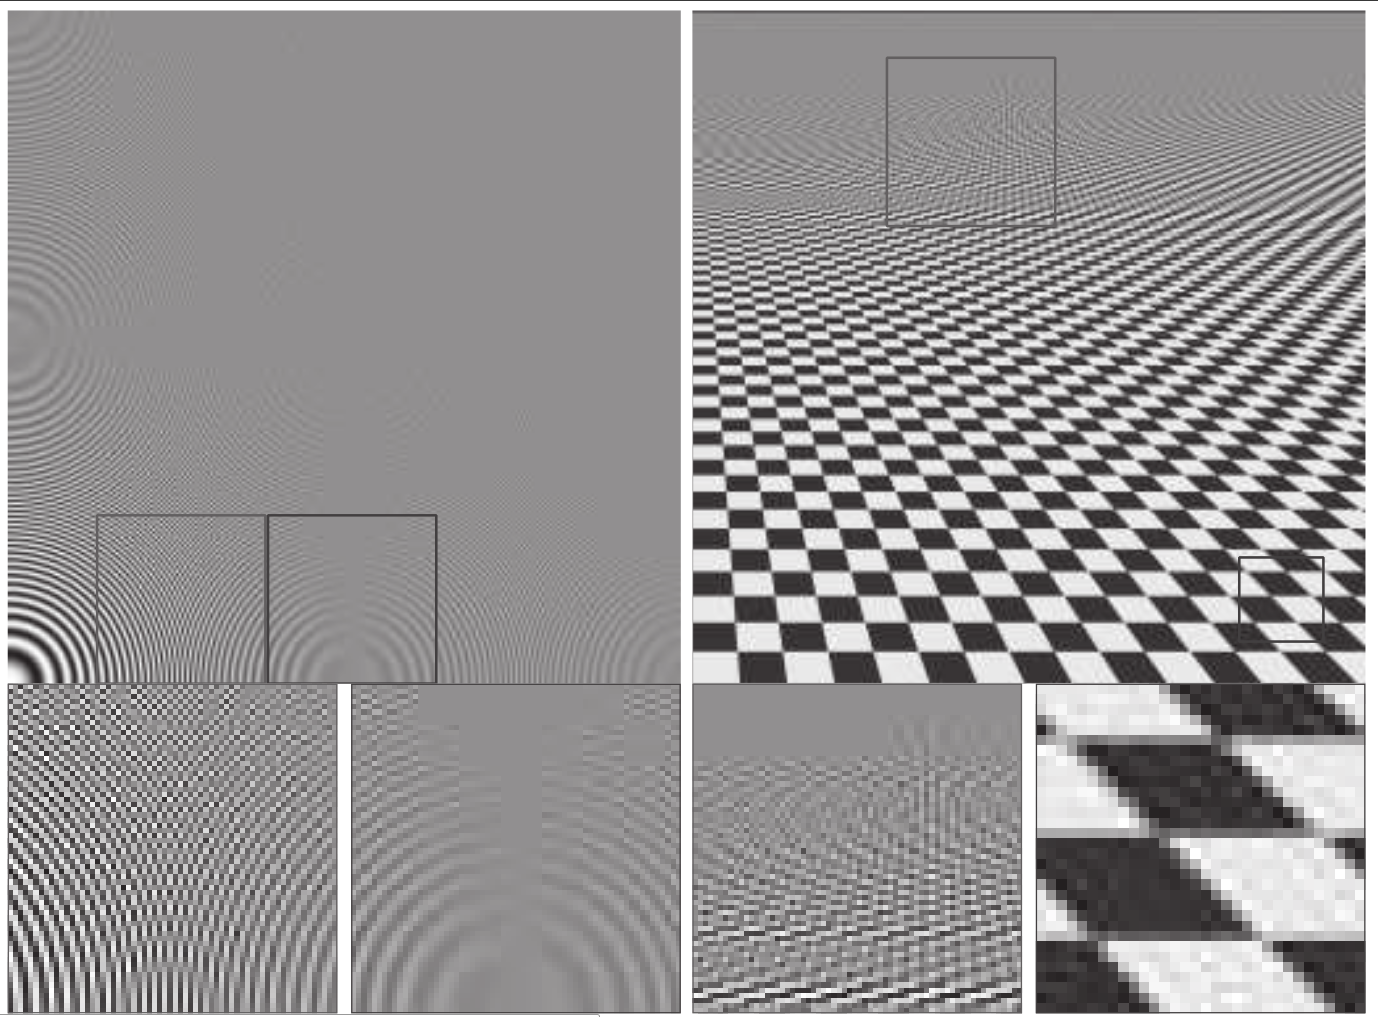
\includegraphics[width=.8\linewidth]{../assets/chapter5_reconstruction_box_result.png}
	\caption{Risultato dell'applicazione del box filter ad un checkeboard pattern}
	\label{chapter5:reconstruction:boxFilterResult}
\end{figure}
\subsection{Gaussian Filter}
\begin{figure}[tb]
	\centering
	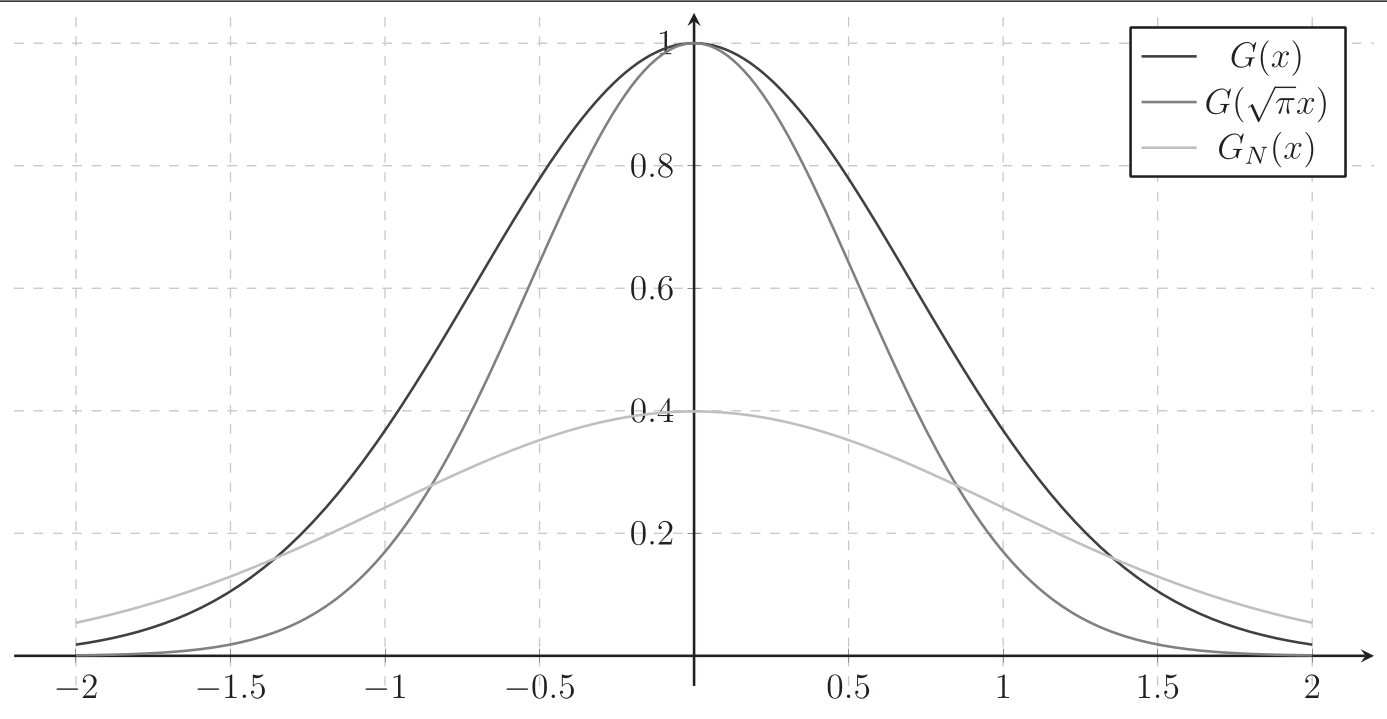
\includegraphics[width=0.8\linewidth, trim=0px 0px 0px 5px, clip]{../assets/chapter5_reconstruction_gaussian.png}
	\caption{Illustrazione di una gaussiana}
	\label{chapter5:reconstruction:gaussian}
\end{figure}
Questo filtro convolve l'immagine non filtrata con un kernel gaussiano. In quanto non presenta lobi negativi, tale filtro sfoca l'immagine originale, 
il che pu\`o essere effetto indesiderato nella ricostruzione. Filtri pi\`u complicati, come il Mitchell-Netvali Filter, qui non trattati 
(si rimanda a \cite{pegoraro}, \cite{pharr}), riescono ad ottenere un risultato di qualit\`a simile al Gaussian Filter, preservandone la sharpness. 
L'equazione di tale filtro
\begin{equation}
	f(x)=G(x;0,\sigma)
\end{equation}
dove 
\begin{align}
	G(x;\mu,\sigma)&=\frac{1}{\sigma\sqrt{2\pi}}e^{-\frac{(x-\mu)^2}{2\sigma^2}}\\
	\fourier{G(x,\mu,\sigma)}&=\frac{e^{\frac{\sigma^2\nu^2}{2}+\iota\mu\nu}}{\sqrt{2\pi}\sqrt{\tfrac{1}{\sigma^2}}\sigma}=
		\frac{e^{\iota\mu\nu}}{\sigma}G\left(\nu;0,\tfrac{1}{\sigma}\right)\\
	\int G(x;\mu,\sigma)\mathrm{d}x&=\frac{1}{2}\left(1+\operatorname{erf}\left(\frac{x-\mu}{\sqrt{2}\sigma}\right)\right)
\end{align}
La funzione di trasferimento del Gaussian Filter \`e dunque
\begin{equation}
	F(\nu)=\frac{1}{\sigma}G\left(x;0,\tfrac{1}{\sigma}\right)
\end{equation}
Per far in modo che il filtro abbia un raggio definito $x_b$ e vada a zero per un valore finito, raffiniamo il filtro come 
\begin{equation}
	f(x)=\left\{\begin{aligned}
		&G(x;0,\sigma)-G(x_b;0,\sigma)\;&|x|<x_b\\
		&0 &\;\;\mathrm{altrimenti}
	\end{aligned}\right.
\end{equation}
Supponendo composizione bidimensionale come separable filter, possiamo campionare ciascuna dimensione separatamente. La CDF calcolata in un punto $x_s$
\begin{equation}
	2\int_0^{x_s}G(x;0,\sigma)-G(x_b;0,\sigma)\mathrm{d}x=\operatorname{erf}\left(\frac{x_s}{\sqrt{2}\sigma}\right)-
		\operatorname{erf}\left(\frac{\-x_b}{\sqrt{2}\sigma}\right)
\end{equation}
Si evince che il suo campionamento risulta essere arduo con Inverse Transform Sampling. Ci sono diverse opzioni
\begin{itemize}[topsep=0pt,noitemsep]
	\item Utilizzare la versione classica del filtro, per il quale $x_s=\sqrt{2}\sigma\operatorname{erf}^{-1}(\xi)$ \cite{pegoraro}
	\item Utilizzare una approssimazione polinomiale o piecewise constant, normalizzarla, e utilizzarla come CDF \cite{pharr}
\end{itemize}
\begin{figure}[tb]
	\centering 
	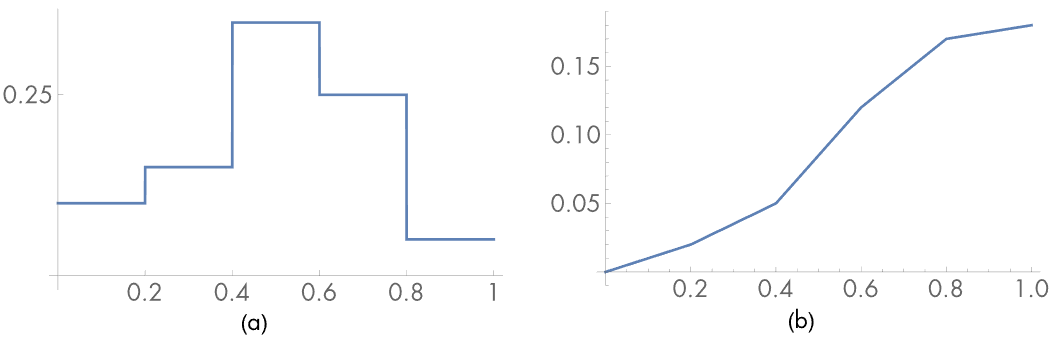
\includegraphics[width=0.8\linewidth]{../assets/chapter5_reconstruction_piecewise.png}
	\caption{Illustrazione funzione definita a tratti. Immagine da \cite{pharr}}
	\label{chapter5:reconstruction:piecewisePDF}
\end{figure}
Tale problema si ripropone nella composizione bidimensionale del Gaussian Filter, il quale nella sua forma classica pu\`o essere campionato mediante 
Inverse Transform Sampling (si rimanda a \cite{pegoraro}).\par
Il metodo alternativo che esaminiamo \`e campionare una approssimazione piecewise della funzione in questione. Esaminiamo una generica funzione 
costante definita in $[0,1)$ con $N$ tratti 1D di equo spessore $\Delta=1/N$, 
\begin{equation}
	f(x)=\left\{\begin{aligned}
		&v_0\;x_0\leq x\leq x_1\\
		&v_1\;x_0\leq x\leq x_2\\
		&\vdots
	\end{aligned}\right.
\end{equation}
\begin{equation}
	c=\int_0^1 f(x)\mathrm{d}x=\sum_{i=0}^{N-1}\frac{v_i}{N}
\end{equation}
Dunque possiamo costruire una PDF da $f(x)$ come $p(x)=\tfrac{f(x)}{c}$. Essendo la PDF una funzione costante definita a tratti, la CDF risultera 
essere una funzione lineare definita a tratti (Figura \ref{chapter5:reconstruction:piecewisePDF})
\begin{align}
	P(x_0)&=0\nonumber\\
	P(x_1)&=\int_{x_0}^{x_1}p(x)\mathrm{d}x=\frac{v_0}{cN}=P(x_0)+\frac{v_0}{cN}\nonumber\\
	\vdots\nonumber\\
	P(x)&=\sum_{j=1}^{i}\left(\frac{v_{j-1}}{cN}\right),\;x\in[x_{i-1},x_i]
\end{align}
Invertire tale funzione consiste nel trovare il valore $x_s$ tale che
\begin{equation*}
	\xi=\int_0^{x_s}p(x)\mathrm{d}x=P(x_s)
\end{equation*}
\begin{figure}[tb!]
	\centering
	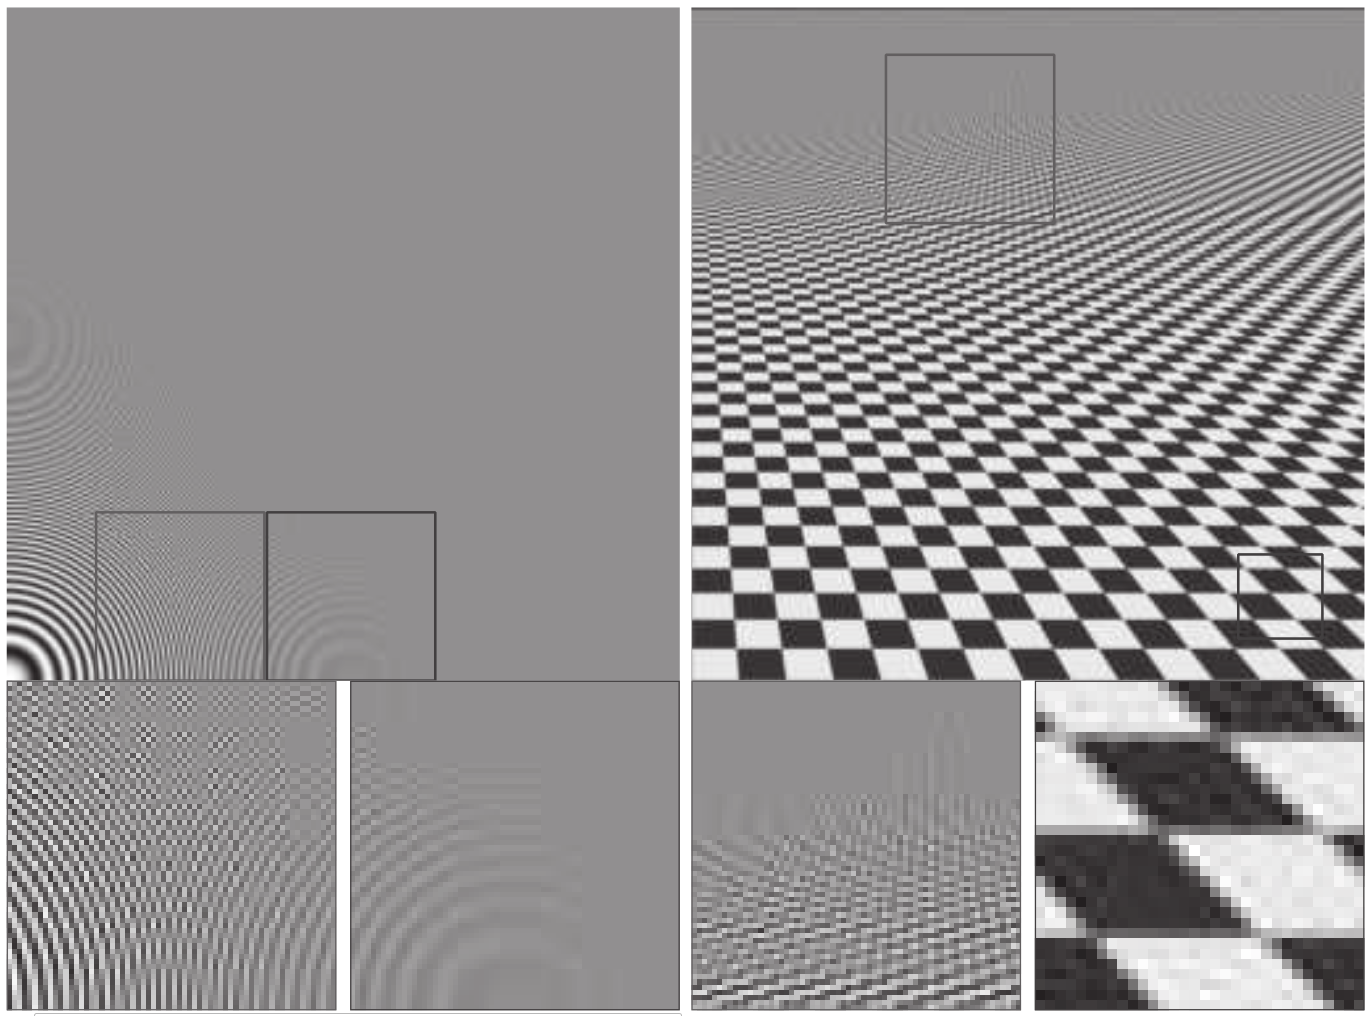
\includegraphics[width=0.75\linewidth]{../assets/chapter5_reconstruction_gaussian_result.png}
	\caption{Risultato di applicazione del Gaussian Filter radiale ad un checkerboard pattern. Immagine da \cite{pegoraro}}
	\label{chapter5:reconstruction:gaussianResult}
\end{figure}
In quanto la CDF \`e crescente, possiamo tradurre tale task nel trovare una coppia di punti $(x_i,x_{i+1})$ tali che $\mathmakebox{P(x_i)\leq\xi}$ e 
$\mathmakebox{\xi\leq P_{i+1}}$ effettuando una ricerca binaria. Dopodich\`e, possiamo calcolare quanto distante $\xi$ \`e dall'estremo inferiore 
dell'intervallo definito dai punti trovati $x_i$, $\Delta\xi=\frac{\xi-x_i}{x_{i+1}-x_i}$, dove si tiene cura di eseguire la divisione solo se
$x_{i+1}>x_i$. Il campione per Inverse Tramsform Sampling pu\`o dunque essere posto pari a 
\begin{equation}
	x_s = x_i + \Delta\xi
\end{equation}
